\chapter{Model Systemu}
\section{System zbiorników}
\indent Przedmiotem rozważań jest system 3 połączonych zbiornkiów. Dwa zbiorniki pełnią rolę rezerwy wody oraz koncentratu. W trzecim odbywa się mieszanie gotowego produktu o zadanym stężeniu. Gotowa mieszanka dozowana jest w odpowieniej ilości do pojemników na taśmie produkcyjnej. Regulacja przepływu pomiędzy zbiornikami odbywa się przy pomocy sterowanych zaworów. Poglądowy schemat procesu znajduje się na rysunku \ref{fig:Proces}.
\begin{figure}[H]
	\centering
	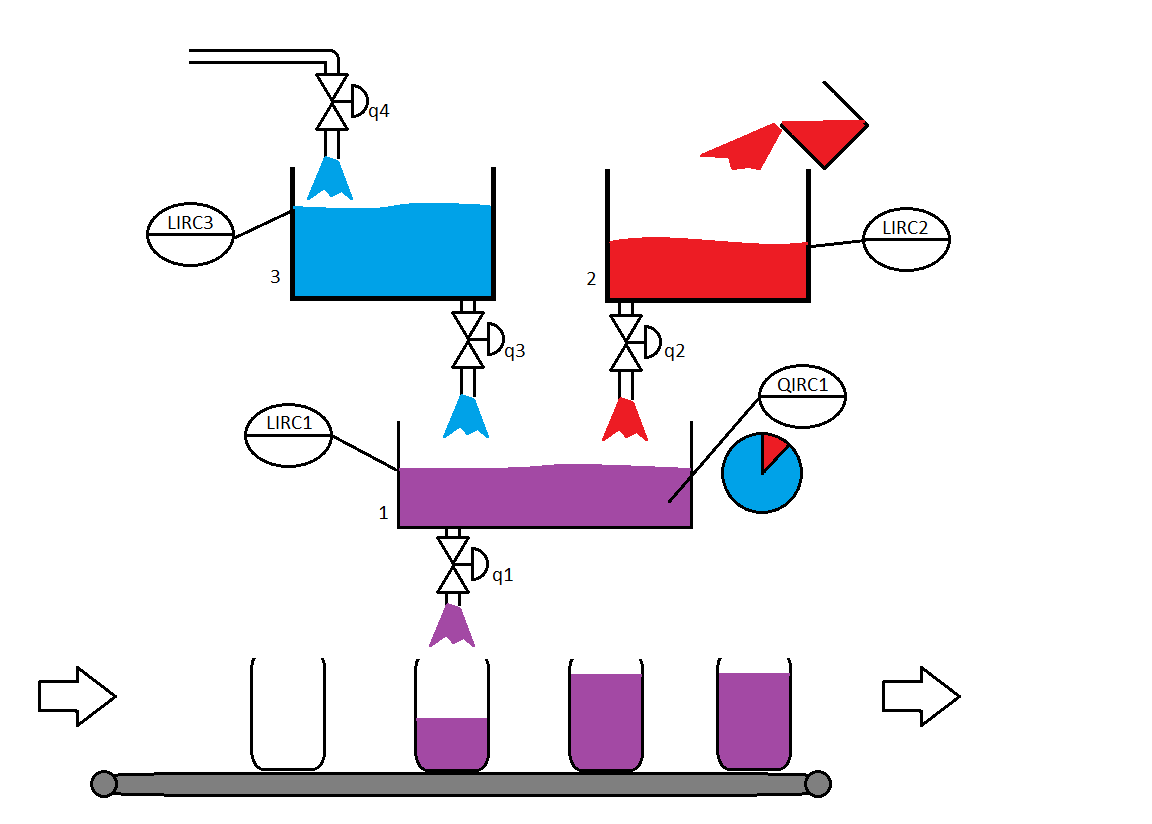
\includegraphics[scale = 0.5]{fig/Proces_schema_updated.png}
	\caption{Schemat procesu.}
	\label{fig:Proces}
\end{figure}

Dynamika procesu do celów symulacji została zamodelowana przy pomocy równań różniczkowych. Zależność prędkości wypływu ze zbuornika od wyskości cieczy została przybliżona zależnością pierwiastkową. Dodatkowo może być ona steowana poprzez stopień otwarcia zaworu. Ostatecznie równiania uzyskują postać:


\begin{align*}\label{rownania_stanu}
\frac{dH_{3}}{dt} &= \frac{1}{\beta(H_{3})} q_{4} v_{4}-\frac{1}{\beta(H_{3})} q_{3} \sqrt{H_{3}} \\
\frac{dH_{2}}{dt} &= \frac{1}{\beta(H_{2})} K-\frac{1}{\beta(H_{2})} q_{2} \sqrt{H_{2}} \\
\frac{dH_{1}}{dt} &= \frac{1}{\beta(H_{1})} q_{3} \sqrt{H_{3}}+\frac{1}{\beta(H_{1})} q_{2} \sqrt{H_{2}}-\frac{1}{\beta(H_{1})} q_{1} \sqrt{H_{1}},
\end{align*}
\begin{align*}
gdzie: &\\
	H_{i} -& \text{poziom w $i$ -tym zbiorniku}\\
	\beta(H_{i}) -& \text{powierzchnia swobodna w $i$ -tym zbiorniku dla poziomu $H_{i}$, w przypadku}\\ & \text{ zbiorników o stałym przekroju } \beta(H_{i})=const \\
	q_{i}  -& \text{stopień otwarcia $i$ -tego zaworu}\\
	v_{4}  -& \text{strumień wody zasilającej zbiornik 3}\\
	K -& \text{dopływ koncentratu do zbiornika 2}\\
\end{align*}
  Na podstawie modelu matematycznego utworzono symulację w środowisku Matlab Simulink. Układ modelu symulacyjnego przedstawiony jest na rysunku \ref{fig:Simulink_diagram}.
\begin{figure}[H]
	\centering
	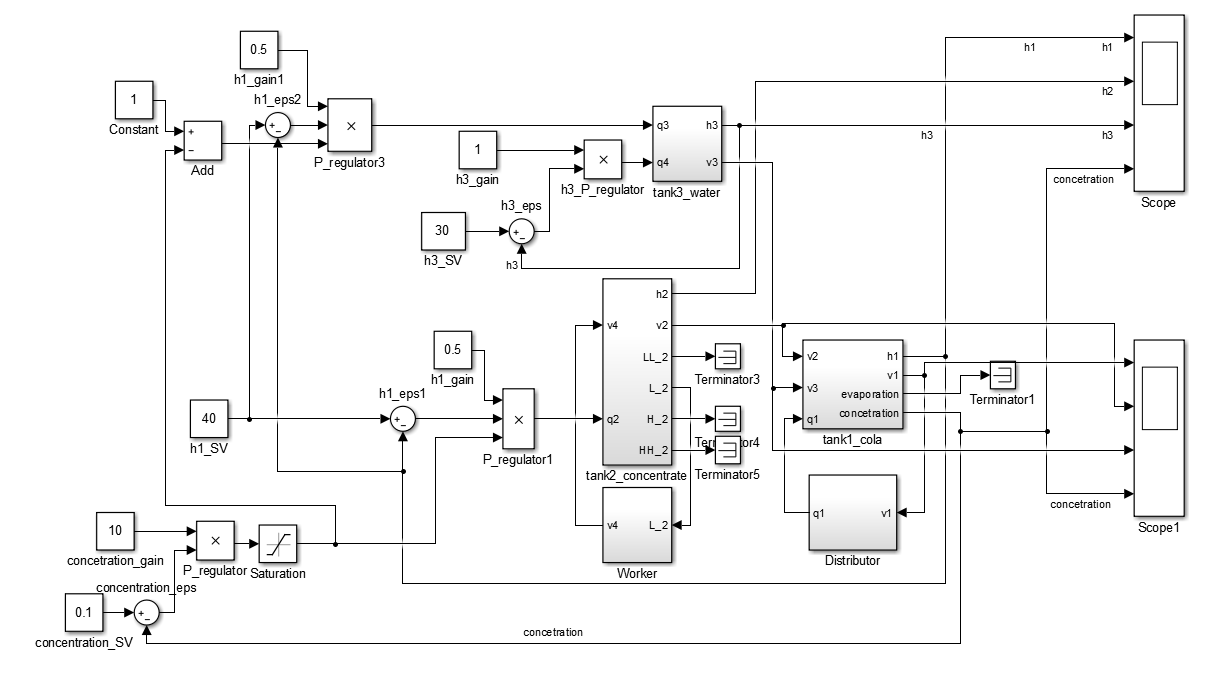
\includegraphics[scale = 0.5]{fig/simulink_diagram.png}
	\caption{Schemat procesu w środowisku Simulink.}
	\label{fig:Simulink_diagram}
\end{figure}



\section{Regulatory}
\subsection{Regulacja poziomu wody w zbiorniku 3}
\indent Regulacja poziomu wody w zbiorniku $H_{3}$ odbywa się poprzez regulator proporcjonalny sterujący stopniem otwarcia zaworu $q_{4}$. Wartość sterowania wyliczana jest na podstawie uchybu pomiędzy wartością zadaną {h3\_SV} a wysokością poziomu wody w zbiorniku h3.
\begin{figure}[H]
	\centering
	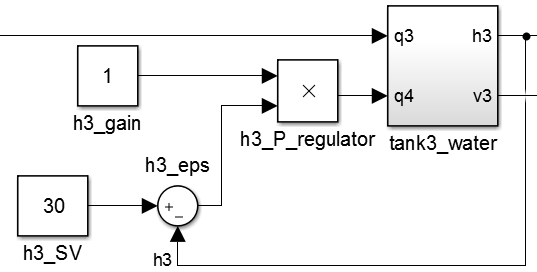
\includegraphics[scale = 0.4]{fig/h3_regulator.png}
	\caption{Schemat regulatora poziomu wody $H_{3}$.}
	\label{fig:h3reg}
\end{figure}
\subsection{Regulacja poziomu koncentratu w zbiorniku 2}
\indent Regulacja poziomu koncentratu w zbiornkiu 2 odbywa się poprzez dolewanie dodatkowych porcji substancji przez pracownika po zgłoszeniu przez system komunikatu o niskim poziomie cieczy w zbiorniku. Aby zamodelować działanie pracownkia, który posiada pewną zwłokę w wykonywaniu działań oraz potrzebuje czasu na przemieszczenie się z dodatkową porcją koncentratu, użyto maszyny stanów. Określono czas reakcji pracownika na komunikat systemowy, czas potrzebny do zabrania kolejnej porcji, oraz czas potrzebny na uzupełnienie koncentratu. Schemat działania pokazano na rysunku \ref{fig:Worker_state}.
\begin{figure}[H]
	\centering
	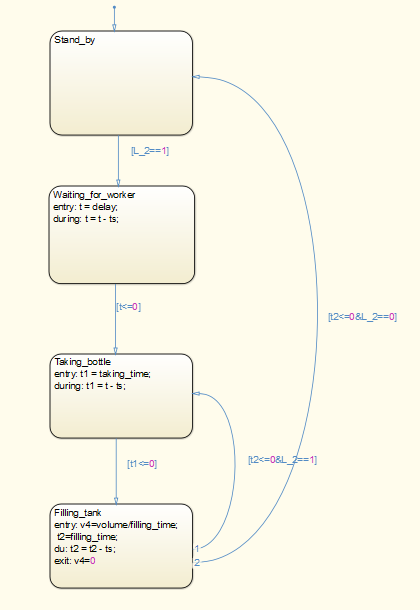
\includegraphics[scale = 0.8]{fig/worker_state.png}
	\caption{Schemat maszyny stanów imitującej działanie pracownika}
	\label{fig:Worker_state}
\end{figure}
\subsection{Regulacja dawkowania wody i koncentratu do zbiornika mieszającego}
\indent Regulacja przepływu wody oraz koncentratu do zbiornika mieszającego odbywa się na podstawie pomiaru wysokości cieczy w zbiorniku 1 oraz na podstawie pomiaru stężenia koncentratu w gotowym produkcie. Regulacja odbywa się w taki sposób aby utrzymać zadany poziom w zbiorniku oraz zadane stężenie gotowego produktu. Schemat działania regulatorów przedstawony został na rysunku \ref{fig:h1reg}. W celu utrzymania zadanych wartości stężenia oraz poziomu $H_{1}$, wykorzystano regulację proporcjonalną dla stopnia otwarcia zaworów $q_{2}$ i $q_{3}$ oraz czynnik proporcjonalny od uchybu stężenia przełączający udział każdego ze sterowań.
\begin{figure}[H]
	\centering
	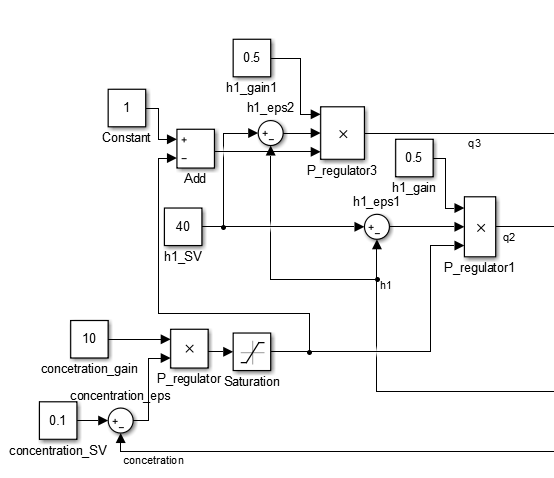
\includegraphics[scale = 0.6]{fig/h1_regulator.png}
	\caption{Schemat regulatora stężenia i poziomu wody $H_{1}$.}
	\label{fig:h1reg}
\end{figure}
\subsection{Regulacja dawkowania gotowej mieszanki ze zbiornika mieszającego}
\indent Regulator odpowiedzialny za napełnianie pojemników gotową mieszanką działa poprzez maksymalne otwarcie wypływu ze zbiornika 1 aż do całkowitego napełnienia się naczynia. Po całkowitym napełnieniu zawór zostaje zamknięty aż do nadejścia kolejnego pojemnika do napełnienia. Jego działanie zostało zaimplementowane przy użyciu maszyny stanów której schemat widnieje na rysunku \ref{fig:Dis_state}.
\begin{figure}[H]
	\centering
	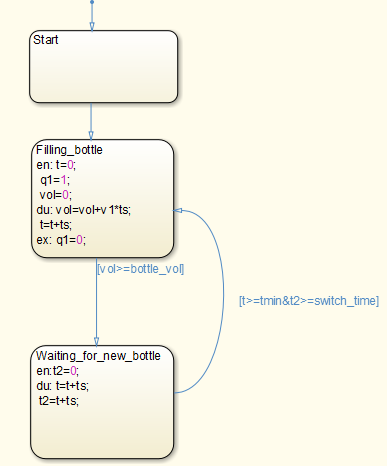
\includegraphics[scale = 0.8]{fig/dis_state.png}
	\caption{Schemat maszyny stanów imitującej działanie dystrubutora}
	\label{fig:Dis_state}
\end{figure}

